\chapter{\selectlanguage{greek}Θεωρητικό υπόβαθρο}
%TODO Write intro

\section{Υπόβαθρο}
\subsection{\selectlanguage{greek}Το \en{CERN}}

To \en{CERN}, διατηρώντας το ακρωνύμιο της αρχικής Γαλλικής ονομασίας του \en{$``$Conseil Européen pour la Recherche Nucléaire$"$}, είναι το μεγαλύτερο σε έκταση πειραματικό κέντρο πυρηνικών ερευνών και ειδικότερα επί της σωματιδιακής φυσικής στον κόσμο. 
Βρίσκεται δυτικά της Γενεύης, στα σύνορα Ελβετίας και Γαλλίας και ιδρύθηκε το 1954 από 12 ευρωπαϊκές χώρες. 
Σήμερα αριθμεί 20 κράτη-μέλη, μεταξύ των οποίων και η Ελλάδα, η οποία είναι και ιδρυτικό μέλος.

\begin{figure}[tph]

\includegraphics[width=0.25\textwidth]{images/CERNlogo.png}
\centering
\caption{Το λογότυπο του \en{CERN}}
\label{img:CERNlogo}
\end{figure}

Η βασική λειτουργία του \en{CERN} είναι η παροχή επιταχυντών σωματιδίων και άλλων υποδομών απαραίτητων για την έρευνα στον τομέα της φυσικής υψηλών ενεργειών και ως αποτέλεσμα έχουν πραγματοποιηθεί πολυάριθμα πειράματα στο \en{CERN} μέσω διεθνών συνεργασιών.

Επίσης, το \en{CERN} αποτελεί τη γενέτειρα του Παγκόσμιου Ιστού (\en{World Wide Web}).
Στην κύρια τοποθεσία του στο \en{Meyrin} βρίσκεται μεγάλη εγκατάσταση ηλεκτρονικών υπολογιστών με ισχυρές υποδομές επεξεργασίας δεδομένων, κυρίως για την ανάλυση των πειραματικών δεδομένων. 
Λόγω της ανάγκης να καταστούν αυτές διαθέσιμες σε εξωτερικούς ερευνητές, υπήρξε ιστορικά ένας σημαντικός κόμβος δικτύου ευρείας περιοχής (\en{Wide Area Network}).

Αρκετά σημαντικά επιτεύγματα στο πεδίο της φυσικής των σωματιδίων έγιναν μέσω πειραμάτων στο \en{CERN}. Αυτά περιλαμβάνουν:
\begin{itemize}
\item 1973: Ανακάλυψη των ουδέτερων ρευμάτων στο θάλαμο φυσαλίδων \en{Gargamelle}.
\item 1983: Ανακάλυψη των μποζονίων $W$ και $Z$ στα πειράματα \en{UA1} και \en{UA2}.
\item 1995: Πρώτη δημιουργία ατόμων αντιυδρογόνου στο πείραμα \en{PS210}.
\item 1999: Ανακάλυψη της άμεσης παραβίασης \en{CP} στο πείραμα \en{NA48}.
\item 2010: Απομόνωση 38 ατόμων αντιυδρογόνου.
\item 2011: Διατήρηση αντιυδρογόνου για πάνω από 15 λεπτά.
\item 2012: Ένα μποζόνιο με μάζα περίπου \SI[per-mode = symbol]{125}{\giga \electronvolt \per  \clight \squared} συνάδει με τον πολυπόθητο μποζόνιο \en{Higgs}.
\end{itemize}


\subsection{\selectlanguage{greek}Ο επιταχυντής \en{CLIC}}


Ο \en{CLIC --- Compact Linear Collider} --- αποτελεί μια μελέτη για ένα μελλοντικό επιταχυντή που θα φτάσει σε πρωτοφανή επίπεδα ενέργειας ηλεκτρόνια και αντισωμάτιά τους, ποζιτρόνια. 
Όταν θα έρχονται σε επαφή μέσω σύγκρουσης, θα αλληλοκαταστρέφονται, απελευθερώνοντας όλη τους την ενέργεια για την παραγωγή νέων σωματιδίων.

\begin{figure}[b]

\includegraphics[trim={12mm 12mm 12mm 12mm},clip=true,width=0.25\textwidth]{images/CLIClogo}
\centering
\caption{Το λογότυπο του \en{CLIC}}
\label{img:CLIClogo}
\end{figure}

Τα ηλεκτρόνια και τα ποζιτρόνια είναι θεμελιώδη σωματίδια και οι συγκρούσεις τους μπορούν να προσφέρουν εξαιρετικά λεπτομερείς πληροφορίες σχετικά με τους νόμους της φύσης. 
Έτσι ο \en{CLIC} θα προσφέρει σημαντικές θεμελιώδεις γνώσεις φυσικής, πέρα από αυτές που είναι διαθέσιμες από το Μεγάλο Επιταχυντή Αδρονίων (\en{Large Hadron Collider --- LHC}) ή από ένα γραμμικό επιταχυντή ηλεκτρονίων/ποζιτρονίων χαμηλότερης ενέργειας, λόγω του μοναδικού συνδυασμού πειραματικής ακρίβειας και υψηλής ενέργειας.

Σε αυτές τις υψηλές ενέργειες, τα ηλεκτρόνια και ποζιτρόνια θα έχαναν ένα τεράστιο μέρος της ενέργειάς τους επιταχυνόμενα σε έναν κυκλικό επιταχυντή σαν τον \en{LHC}. 
Επομένως, τα σωματίδια πρέπει να επιταχυνθούν σε δύο γραμμικούς επιταχυντές που αντικρίζουν ο ένας τον άλλο έτσι, ώστε οι δέσμες να συγκρούονται στον κεντρικό ανιχνευτή. 
Αυτό συνεπάγεται ότι τα σωματίδια πρέπει να αποκτήσουν την ενέργειά τους από ένα και μόνο πέρασμα τους μέσα από τις κοιλότητες επιτάχυνσης.

\begin{figure}[tph]
\includegraphics[width=0.6\textwidth]{images/CLIC-twobeam.jpg}
\centering
\caption{Το σύστημα δύο δεσμών του \en{CLIC}}
\label{img:CLICtwobeamscheme}
\end{figure}

Ο \en{CLIC} έχει σχεδιαστεί για να κατασκευαστεί σε στάδια αυξανόμενης ενέργειας για σύγκρουση: ξεκινώντας από \SI{360}{\giga \electronvolt}, περίπου \SI{1.4}{\TeV}, και μέχρι την τελική ενέργεια των \SI{3}{\TeV}. 
Προκειμένου να επιτευχθεί αυτή η ενέργεια με ένα ρεαλιστικό και οικονομικά αποδοτικό τρόπο, η αύξηση της επιτάχυνσης πρέπει να είναι πολύ υψηλή.
Ο \en{CLIC} αποσκοπεί σε επιτάχυνση των \SI[per-mode = symbol]{100}{\mega \volt \per \metre}, 20 φορές υψηλότερη από αυτή του \en{LHC}.

Για να επιτευχθεί αυτό, χρησιμοποιείται μια καινοτόμα μέθοδος επιτάχυνσης, όπου εξάγεται ενέργεια από μια δέσμη πολύ μεγάλης έντασης που περιέχει σχετικά χαμηλής ενέργειας ηλεκτρόνια (Δέσμη Οδηγός)  και χρησιμοποιείται για την επιτάχυνση της χαμηλότερης σε ένταση Κύρια Δέσμης (\en{Main Beam}) σε πολύ μεγάλη ενέργεια.

Αυτή η Δέσμη Οδηγός (\en{Drive Beam}) επιβραδύνεται σε ειδικές Διατάξεις Εξαγωγής και Mεταφοράς Ισχύος --- \en{Power Extraction and Transfer Structures (PETS)}, και η παραγόμενη \en{RF} ισχύς μεταφέρεται στην κύρια δέσμη. 
Αυτό οδηγεί σε μια πολύ απλή διάταξη σήραγγας χωρίς ενεργά \en{RF} μέρη (δηλ. \en{klystrons}).

\begin{figure}[tph]
\includegraphics[width=\textwidth]{images/CLIC-layout.jpg}
\centering
\caption{Το σχεδιάγραμμα του \en{CLIC}}
\label{img:CLIClayout}
\end{figure}

\begin{figure}[tph]
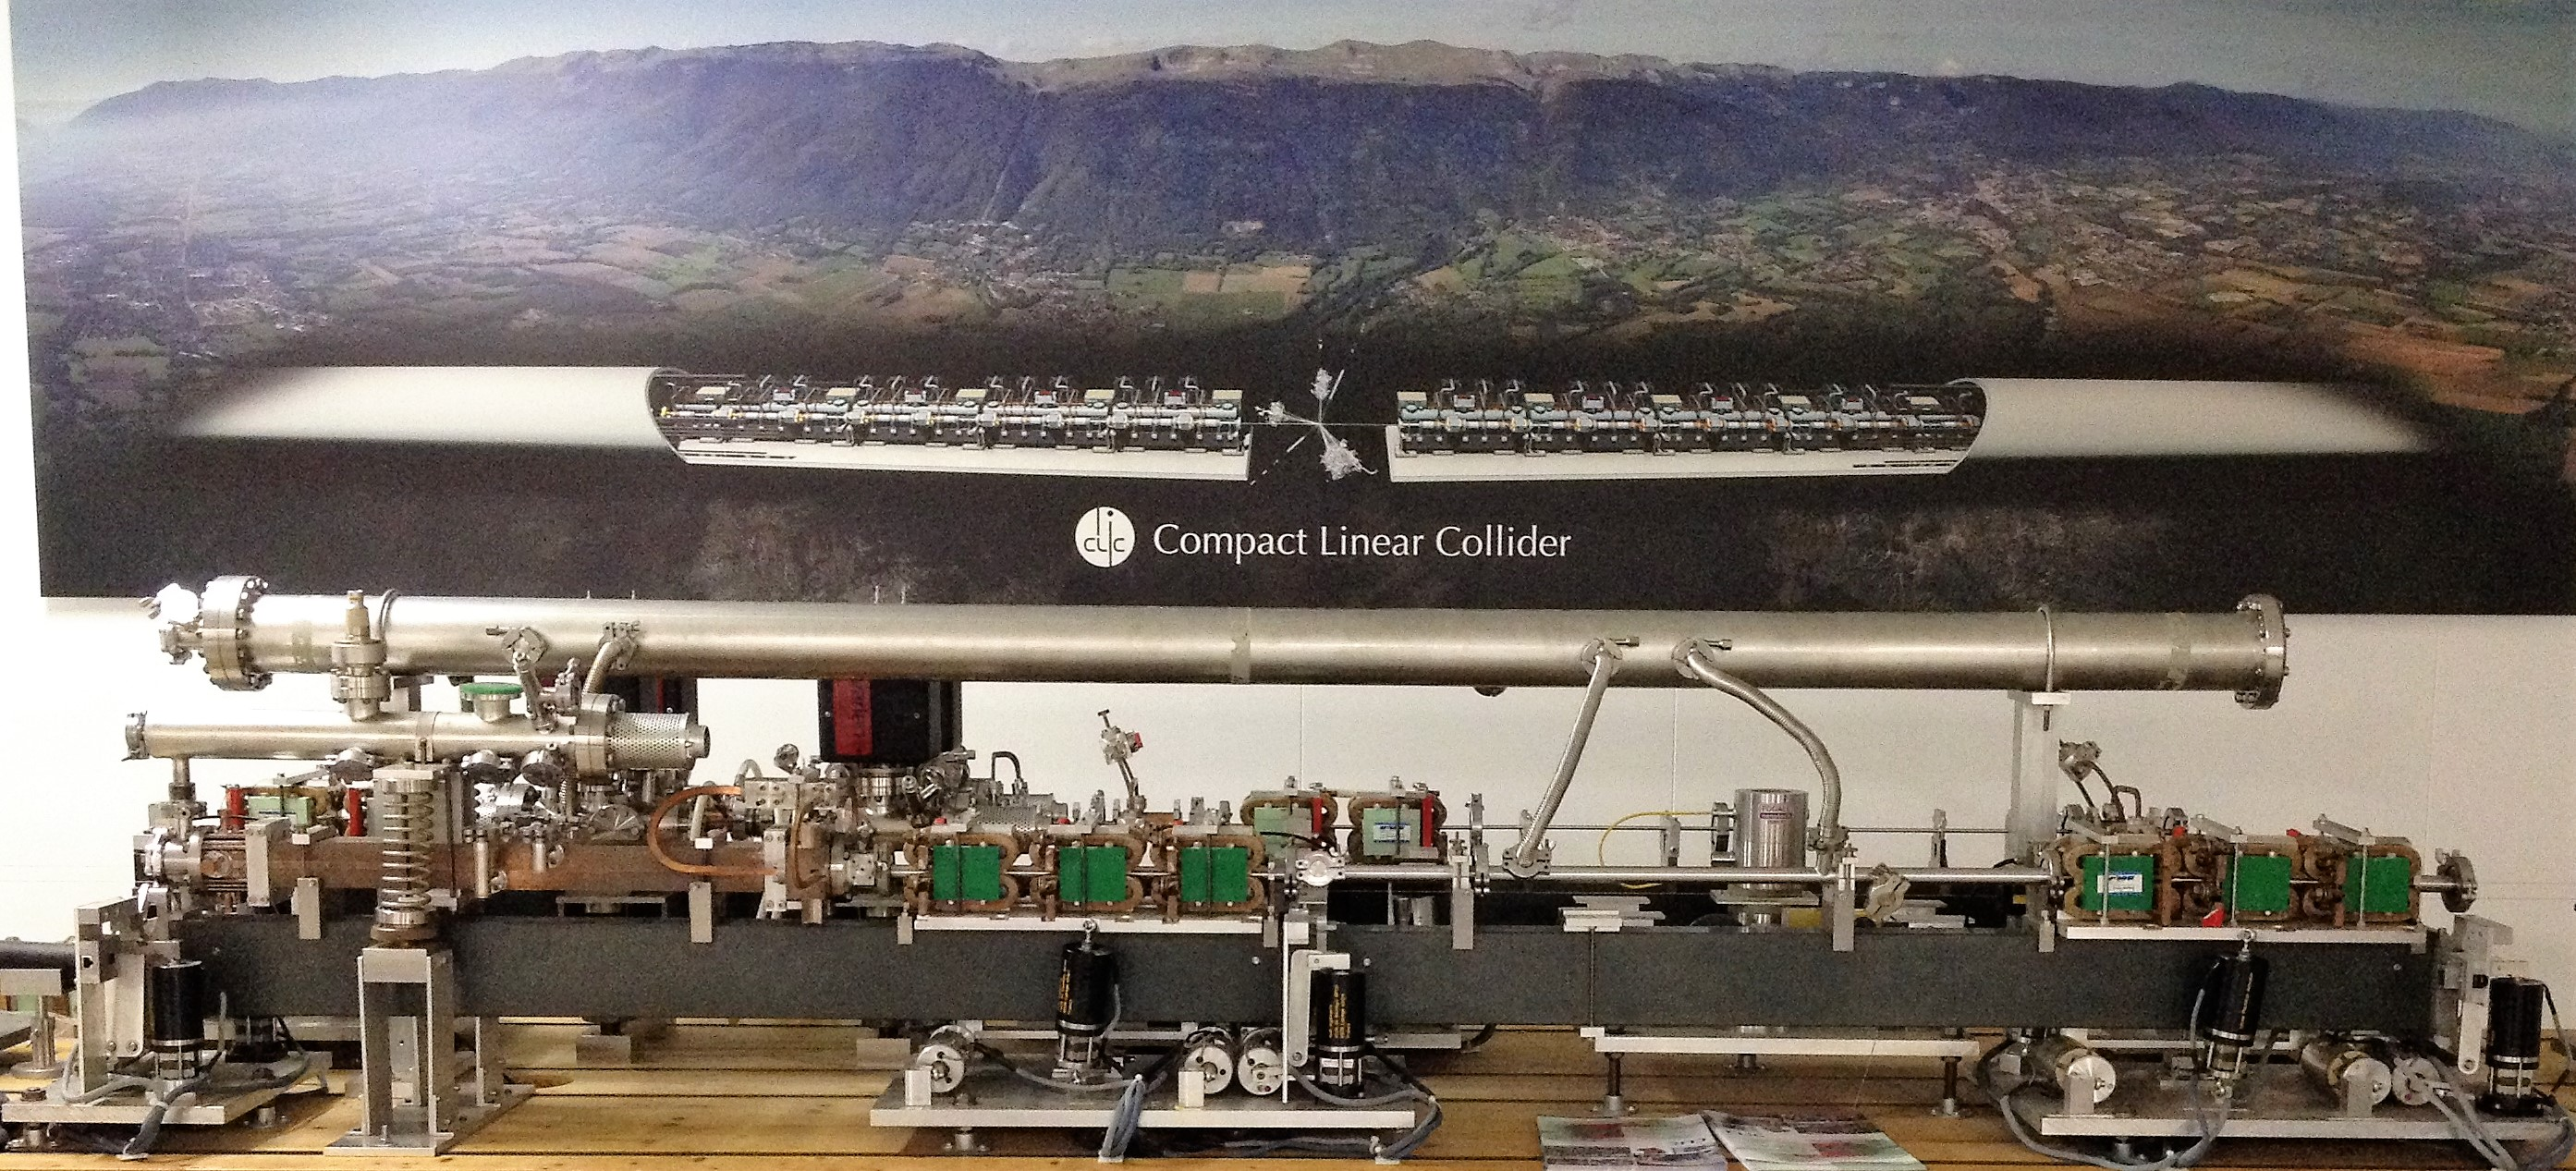
\includegraphics[width=\textwidth]{images/CLIC-maquette}
\centering
\caption[Η μακέτα του \en{CLIC}]{Η μακέτα του \en{CLIC} που βρίσκεται στο κτήριο δοκιμών \en{CLIC Test Facility 3 (CTF3)} του \en{CERN}}
\label{img:CLIClmaquette}
\end{figure}

Ο \en{CLIC} είναι μία από τις επιλογές για έναν μελλοντική επιταχυντή κατασκευασμένο στο \en{CERN}. 
Η τελική απόφαση κατασκευής θα εξαρτηθεί από τα μελλοντικά αποτελέσματα του \en{LHC}.

\begin{figure}[tph]
    \begin{subfigure}{0.5\textwidth}
		\centering
		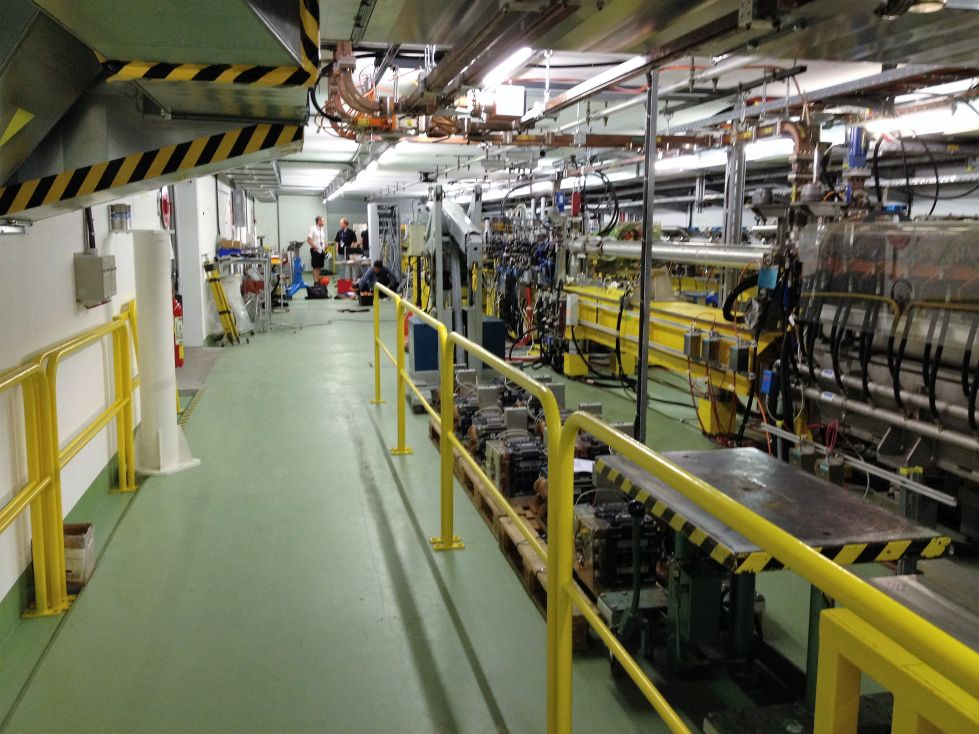
\includegraphics[width=.9\linewidth]{images/CLIC-CTF3-overview.jpg}
    \end{subfigure}
	~
    \begin{subfigure}{0.5\textwidth}
		\centering
		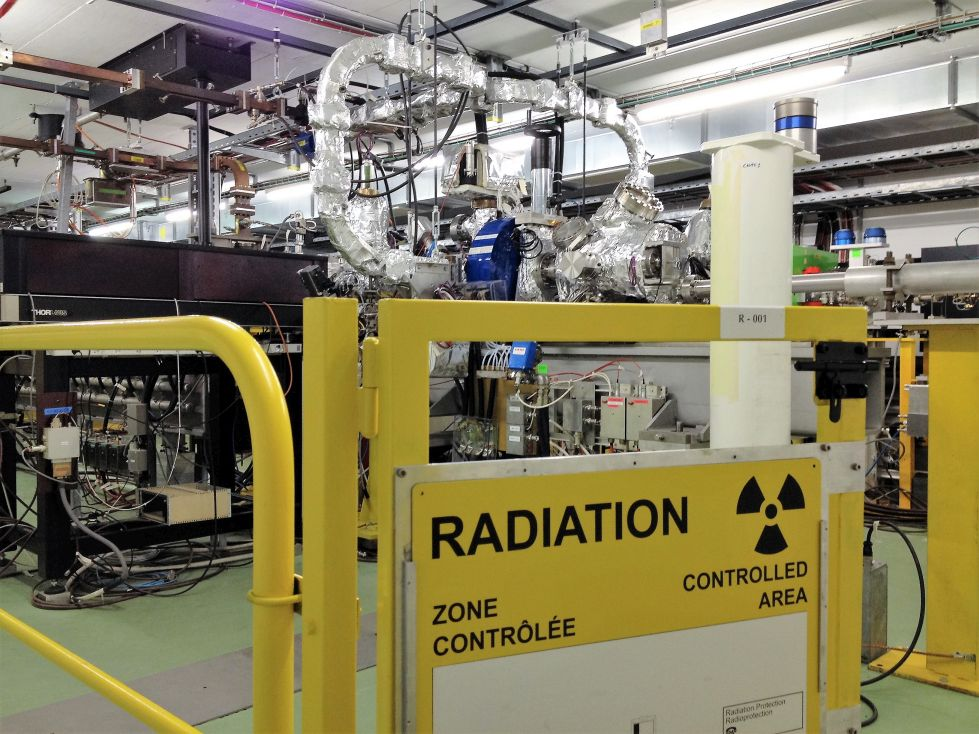
\includegraphics[width=.9\linewidth]{images/CLIC-CTF3-radiation.jpg}
    \end{subfigure}
	\par\bigskip
    \begin{subfigure}{0.5\textwidth}
		\centering
		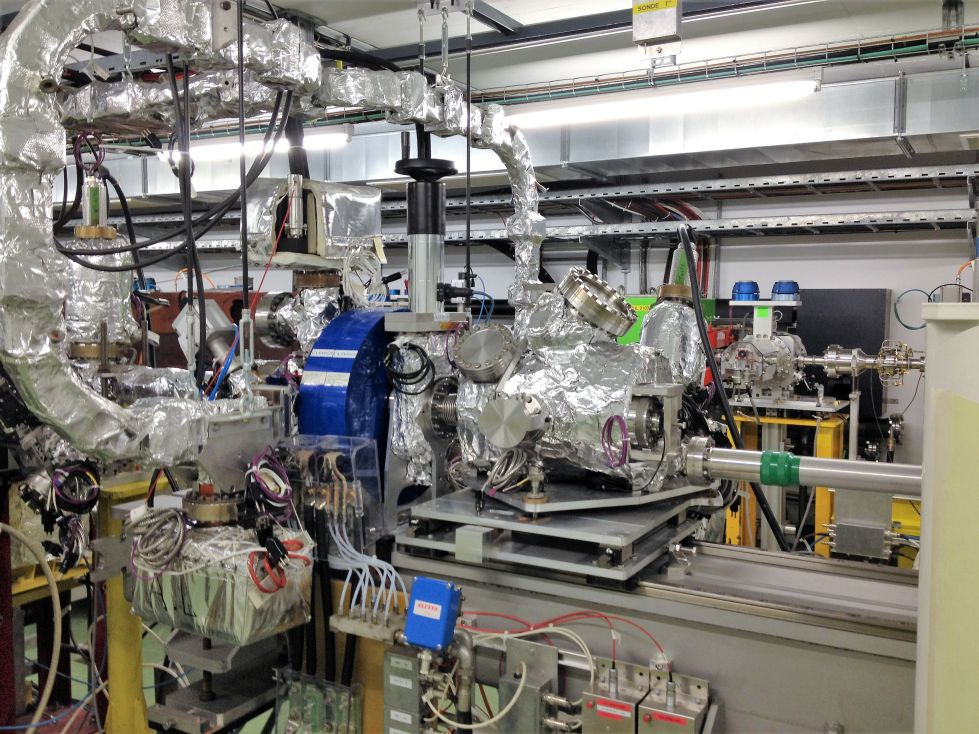
\includegraphics[width=.9\linewidth]{images/CLIC-CTF3-img1.jpg}
    \end{subfigure}        
	~
    \begin{subfigure}{0.5\textwidth}
		\centering
		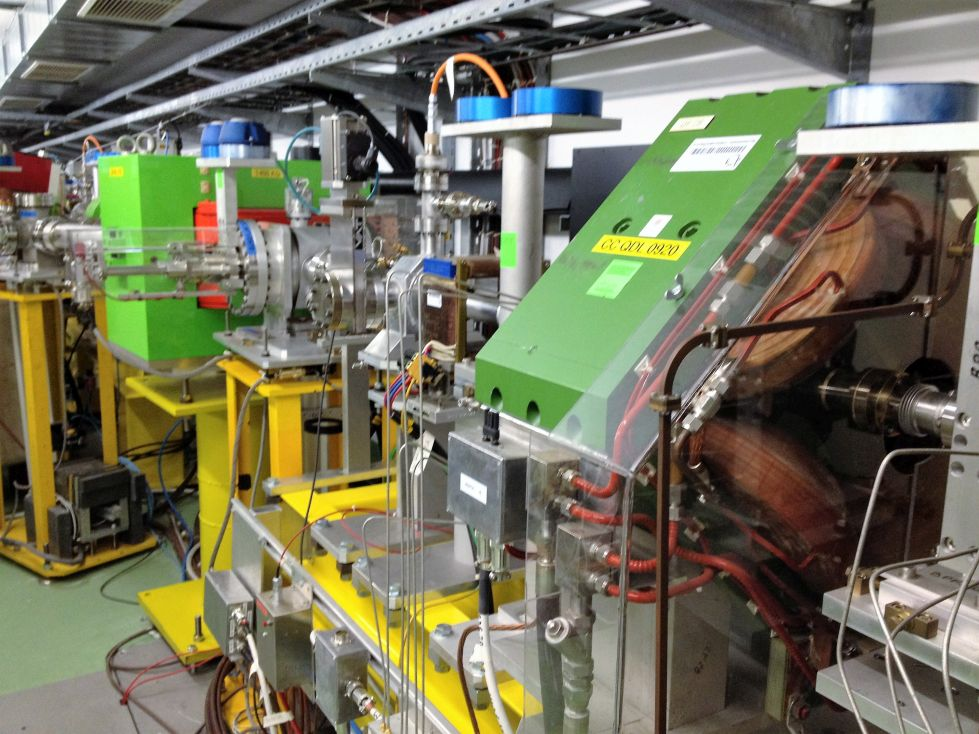
\includegraphics[width=.9\linewidth]{images/CLIC-CTF3-img2.jpg}
    \end{subfigure}
	\par\bigskip
    \begin{subfigure}{0.5\textwidth}
		\centering
		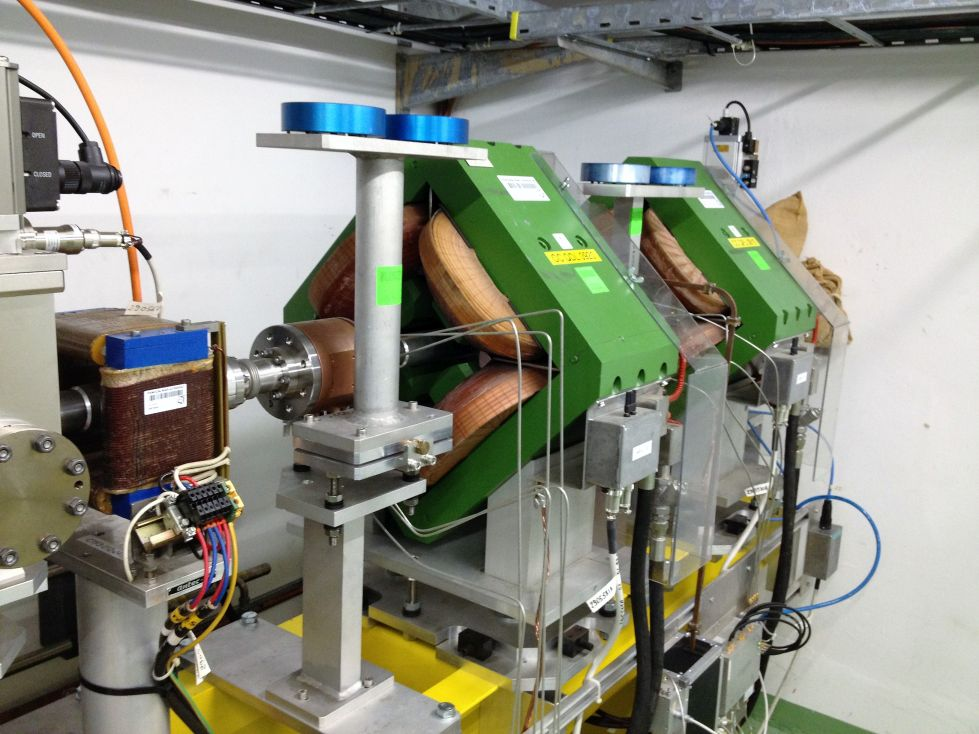
\includegraphics[width=.9\linewidth]{images/CLIC-CTF3-img3.jpg}
    \end{subfigure}        
	~
    \begin{subfigure}{0.5\textwidth}
		\centering
		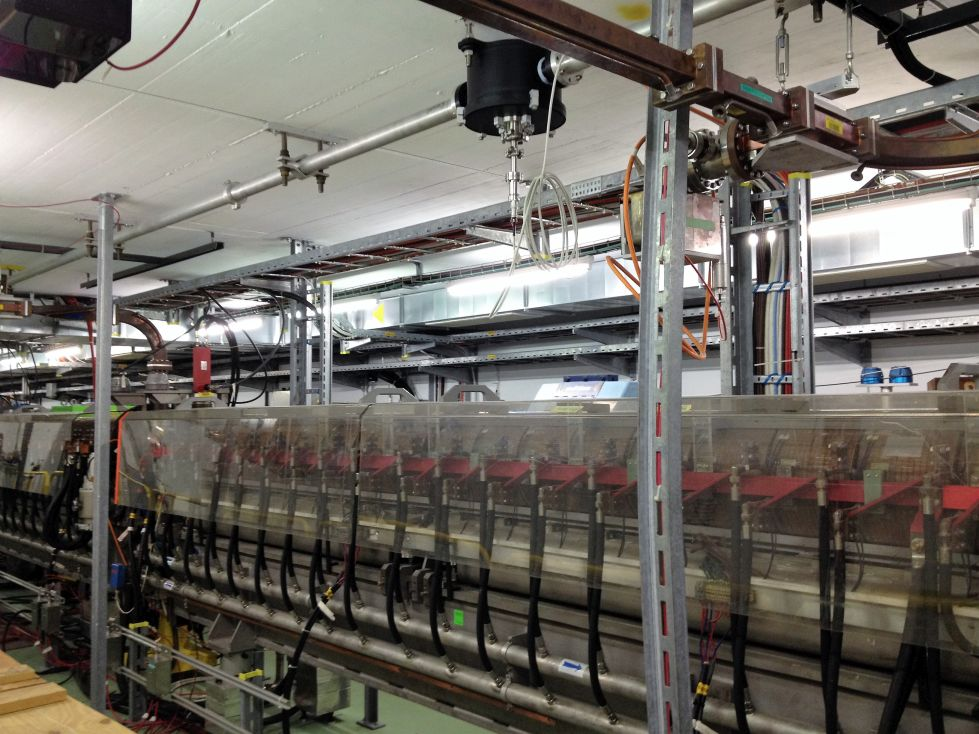
\includegraphics[width=.9\linewidth]{images/CLIC-CTF3-img4.jpg}
    \end{subfigure}
    
\caption[Εικόνες από το \en{CLIC Testing Facility 3}]
{Εικόνες από το \en{CLIC Testing Facility 3 (CTF3)}, όπου γίνονται δοκιμές για το \en{CLIC}. 
Λόγω της φύσης των δοκιμών, το \en{CTF3} θεωρείται \en{$``$radiation controlled zone$"$} και για την είσοδο κάποιου στο χώρο απαιτείται να έχει περάσει 7-ωρη εκπαίδευση (\en{radiation training}) και να φέρει ειδικό δοσίμετρο κατά την επίσκεψη}
\label{img:CLIC-CTF3}        
\end{figure}



\section{\selectlanguage{greek}Ο \en{Electron Beam Scanner}}

\subsection{Εισαγωγή}

Όπως αναφέρεται και προηγουμένως, ο \en{CLIC} αποσκοπεί σε επιτάχυνση των \SI[per-mode = symbol]{100}{\mega \volt \per \metre} και χρησιμοποιεί την καινοτομία των δύο δεσμών για να πετύχει αυτό το στόχο. 
Ως εκ τούτου, είναι απαραίτητο η Δέσμη Οδηγός (\en{Drive Beam}) να έχει πολύ μεγάλη ένταση, το οποίο καθιστά πρόκληση τη μέτρηση της χωρικής έντασης (προφίλ) της δέσμης αυτής. 
Επεμβατικές μέθοδοι, όπως για παράδειγμα το \en{wire scanner}, χρησιμοποιούνται ευρέως σε επιταχυντές. Όμως λόγω της έντασης της δέσμης θα καταστρέφονταν. 
Έτσι οδηγούμαστε στην αναζήτηση νέων μη επεμβατικών μεθόδων για την κάλυψη αυτού του κενού.

Μια μη επεμβατική μέθοδος που εξετάζεται είναι η μέθοδος του \en{Electron Beam Scanner}, όπου μια δέσμη ανίχνευσης (\en{probe beam}) στέλνεται κάθετα προς τη Δέσμη Οδηγό (\en{Drive Beam}). 
Ανιχνεύοντας τη δέσμη ανίχνευσης και μετρώντας την εκτροπή της σε σχέση με την αρχική της θέση, είναι εφικτός ο υπολογισμός του προφίλ της Δέσμης Οδηγού.

Ανιχνευτές \en{Electron Beam Scanner} έχουν χρησιμοποιηθεί στο παρελθόν σε άλλους επιταχυντές που έχουν συνεχείς και πολύ μακριές δέσμες, όπου η κατανομή του φορτίου θεωρείται σταθερή κατά τη μέτρηση.
Η Δέσμη Οδηγός του \en{CLIC} θα έχει δέσμες μήκους μόλις \num{12} \en{picoseconds}. 
Αυτό δημιουργεί πρόσθετες προκλήσεις για τη λειτουργία του \en{Electron Beam Scanner}.
Στην παρούσα εργασία θα εξετάσουμε τη λειτουργία ενός \en{Electron Beam Scanner} σε επιταχυντή μου το μήκος της δέσμης είναι σημαντικά μικρότερο από το χρόνο σάρωσης της δέσμης ανίχνευσης. 
Συγκεκριμένα, η περίπτωση όπου το μήκος της δέσμης είναι μικρότερο από το χρόνο που απαιτείται για ένα σωματίδιο της δέσμης ανίχνευσης να διασχίσει τη κύρια δέσμη είναι δύσκολο να μοντελοποιηθεί αναλυτικά. 
Δημιουργήθηκε για αυτό το σκοπό ένα περιβάλλον προσομοίωσης για να προσομοιωθεί αυτή η κατάσταση.

\subsection{Σχετική βιβλιογραφία} %TODO find a better title 
Ακολουθώντας την αρχική έρευνα από τους \en{Pasour} και \en{Ngo} \cite{Pasour1992}, ανιχνευτές \en{Electron Beam Scanner} έχουν χρησιμοποιηθεί επιτυχώς για την μέτρηση του εγκάρσιου προφίλ δέσμης σε διάφορους επιταχυντές, όπως τον δακτύλιο \en{Spallation Neutron Source (SNS)} στο \en{Oak Ridge National Laboratory} \cite{Aleksandrov2005} \cite{Blokland2009} και τη δέσμη \en{NTX} στο \en{Lawrence Berkeley National Laboratory} \cite{Roy2005}. 
Αυτοί οι επιταχυντές έχουν μεγάλο μήκος δέσμης εκατοντάδων \en{nanoseconds}. 
Έτσι, η εγκάρσια κατανομή φορτίου μπορεί να θεωρηθεί σταθερή κατά τη μέτρηση.

Ο \en{Electron Beam Scanner} δουλεύει μετρώντας την εκτροπή της δέσμης ανίχνευσης που αποτελείται από χαμηλής ενέργειας ηλεκτρόνια, καθώς αυτά διαπερνούν κάθετα την κύρια δέσμη (Σχήμα \ref{fig:beam-deflection}).
Για την απεικόνιση επιλέξαμε σε αυτή την εργασία ότι μετράμε το εγκάρσιο προφίλ, και ότι η δέσμη οδηγός ταξιδεύει οριζοντίως. 
Φυσικά, το προφίλ μπορεί να μετρηθεί σε κάθε άξονα στρέφοντας τη διάταξη. 


\begin{figure}[tph]
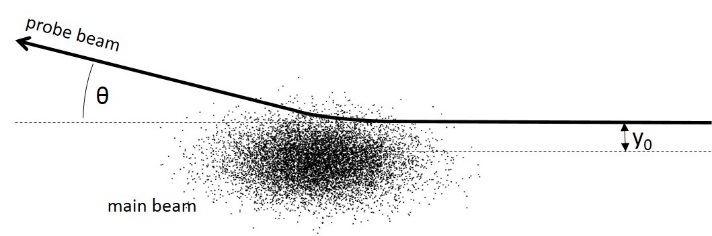
\includegraphics[width=0.8\textwidth]{figures/Beam-deflection}
\centering
\caption{Εκτροπή δέσμης ανίχνευσης από την μετρούμενη δέσμη}
\label{fig:beam-deflection}
\end{figure}

Η γωνία απόκλισης $\theta$ της δέσμης οδηγού μετράται για διαφορετικές τιμές ύψους $y_0$, και το προφίλ της κύριας δέσμης $\delta (y)$ είναι ανάλογο του διαφορικού  \cite{Blokland2009}

\begin{equation} \label{eq:transverseProfile}
\frac{\dd{} |\theta|}{\dd y_0} \propto \delta (y)
\end{equation}

Η σταθερά αναλογίας εξαρτάται από την ενέργεια της δέσμης ανίχνευσης. 
Εδώ έχουν γίνει οι εξής απλοποιητικές υποθέσεις:
\begin{enumerate}
\item Η απόκλιση είναι μικρή
\item Η μεταβολή ενέργειας της δέσμης ανίχνευσης είναι αμελητέα 
\item Η επίδραση του μαγνητικού πεδίου της κύριας δέσμης είναι πολύ μικρότερη από αυτή του ηλεκτρικού πεδίου
\end{enumerate} 

Για να μετρηθεί η γωνία απόκλισης για διαφορετικά $y_0$ σε μία εικόνα, σαρώνεται διαγώνια η αρχική θέση της δέσμης οδηγού. 


Ένας \en{Electron Beam Scanner} έχει επίσης χρησιμοποιηθεί στο \en{Budker Institute for Nuclear Physics} για τη μέτρηση πολύ κοντύτερων δεσμών στον επιταχυντή \en{VEPP-5} \cite{Logatchov2006}, με μήκος δέσμης της τάξης μεγέθους του \SI{1}{\nano \second}.
Σε αυτή την περίπτωση η εγκάρσια κατανομή φορτίου μεταβάλλεται κατά τη μέτρηση.
Έτσι, όχι μόνο η απόκλιση της δέσμης στην κάθετη διεύθυνση δεν είναι σταθερή, αλλά υπάρχει και πρόσθετη απόκλιση κατά μήκος του άξονα της δέσμης του επιταχυντή, λόγω του κατά μήκος διαφορικού του φορτίου.

Σε τέτοιες περιπτώσεις, μια (μη σαρωμένη) δέσμη ανίχνευσης αποκλίνει έτσι, ώστε να το ίχνος να αφήνει μια έλλειψη στην οθόνη κάθε φορά που περνά μια δέσμη.
Ο λόγος των αξόνων της έλλειψης καθορίζεται από το μήκος της δέσμης και το φορτίο.
Ολόκληρο το διαμήκες προφίλ μπορεί να υπολογιστεί μετρώντας την ένταση της δέσμης ανίχνευσης γύρω από την έλλειψη \cite{Logatchov1999}.
Μετρώντας έναν αριθμό ελλείψεων με διαφορετικές αρχικές θέσεις δίνεται το εγκάρσιο προφίλ, παίρνοντας τη μέγιστη απόκλιση κάθε έλλειψης και εφαρμόζοντας τη σχέση \ref{eq:transverseProfile}.
Έτσι μπορούμε να μετρήσουμε το διαμήκες και το εγκάρσιο προφίλ με μία μόνο συσκευή.


Στην παρούσα εργασία θα εξετάσουμε τη λειτουργία ενός \en{Electron Beam Scanner} σε επιταχυντή μου το μήκος της δέσμης είναι σημαντικά μικρότερο από το χρόνο σάρωσης της δέσμης ανίχνευσης. 
Συγκεκριμένα, η περίπτωση όπου το μήκος της δέσμης είναι μικρότερο από το χρόνο που απαιτείται για ένα σωματίδιο της δέσμης ανίχνευσης να διασχίσει τη κύρια δέσμη είναι δύσκολο να μοντελοποιηθεί αναλυτικά. 
Η πλήρωση αυτής της συνθήκης εξαρτάται από διάφορους παράγοντας, όπως την ενέργεια της δέσμης ανίχνευσης και το μέγεθος της μετρούμενης δέσμης, αλλά μπορεί να ειπωθεί κατά προσέγγιση ότι εφαρμόζεται σε δέσμες με μήκος μικρότερο των \SI{100}{\pico \second}.

Ένα παράδειγμα τέτοιας δέσμης είναι ο προτεινόμενος επιταχυντής \en{Compact Linear Collider (CLIC)}. 
Η δέσμη οδηγός του \en{CLIC} θα επιταχύνει μια δέσμη ηλεκτρονίων υψηλής έντασης έως τα \SI{2.4}{\giga \electronvolt} \cite{Aicheler2012}.
Ο επιταχυντής της δέσμης οδηγού θα είναι γραμμικός επιταχυντής των \SI{1}{\giga \hertz}.
Θα εισάγεται σε εναλλασσόμενα δοχεία, δίνοντας κενό μεταξύ των δεσμών (\en{bunch spacing}) \SI{2}{\nano \second}.
Στο τέλος του γραμμικού επιταχυντή, θα χρησιμοποιείται ένα σύστημα πολλαπλασιασμού συχνότητας \cite{Biscari2009} για να μειώσει το κενό μεταξύ των δεσμών στα \SI{0.083}{\nano \second}, πολλαπλασιάζοντας έτσι το ρεύμα κατά \num{24} και μειώνοντας το μήκος του παλμού κατά τον ίδιο συντελεστή.
Έπειτα, η ενέργεια της δέσμης οδηγού θα μεταφέρεται στην κύρια δέσμη με τη χρήση ειδικά σχεδιασμένων συζευγμένων κοιλοτήτων που επιτρέπουν την επιτάχυνση με ρυθμό που φτάνει πάνω από \SI[per-mode = symbol]{100}{\mega \volt \per \meter} \cite{Degiovanni2014}.

\begin{table}[tph]
\centering
	\begin{tabular}{l c}
		\hline
		\en{Bunch population}	& \SI{5e10}{\electrons} \\ \hline
		\en{Transverse Emittance}	& \SI{100}{\nano \meter \radian} \\\hline
		\en{Bunch length / spacing}	& \SI{13}{\pico \second} / \SI{2}{\nano \second} \\\hline
		\en{Pulse length}	& \SI{140}{\micro \second} \\\hline
		\en{Pulse Population}		& \SI{3e15}{\electrons} \\\hline
		\en{Repetition Frequency}	& \SI{50}{\Hz} \\\hline
	\end{tabular}
\caption[Σχετικές παράμετροι για την Δέσμη Οδηγό του επιταχυντή \en{CLIC}]{Σχετικές παράμετροι για την Δέσμη Οδηγό του επιταχυντή \en{CLIC} \protect{\cite{Aicheler2012}}}
\label{tab:parameters}
\end{table}

Το εγκάρσιο προφίλ της δέσμης θα πρέπει να μετράται σε διάφορα σημεία κατά μήκος του γραμμικού επιταχυντή, και μη επεμβατικοί μετρητές προφίλ αναπτύσσονται για αυτό το σκοπό.
Οι μετρητές πρέπει να έχουν ανάλυση \SI{100}{\micro \meter} ή καλύτερη, ώστε να μετράει το ελάχιστο μέγεθος ακτίνας κατά τη διάρκεια \en{quad scans}.
Επεμβατικές μέθοδοι, όπως οθόνες \en{OTR (Optical Transition Radiation)} μπορούν να εγκατασταθούν παράλληλα για βαθμονόμηση, αλλά για χρήση μόνο κατά τη διάρκεια της λειτουργίας με μειωμένο μήκος παλμών.

\subsection{Θεωρητική ανάλυση του \en{Electron Beam Scanner}} \label{sub:EBS-model}
Η λεπτή δέσμη ανίχνευσης κινείται κατά τον άξονα $X$, είναι κάθετη στην κίνηση της σχετικιστικής κίνησης της κύριας δέσμης (άξονας $Z$), με παράμετρο απόκλισης $\rho$ (Σχήμα \ref{fig:ellipse-EBS}).

\begin{figure}[tph]
	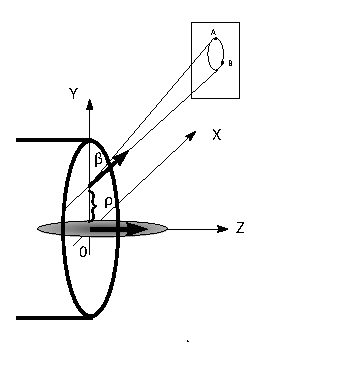
\includegraphics[width=0.6\textwidth]{figures/Logatchov1999-EBS}
	\centering
	\caption{Διαδικασία ανίχνευσης της χαρακτηριστικής έλλειψης της δέσμης}
	\label{fig:ellipse-EBS}
\end{figure}

Τα αποτελέσματα της σάρωσης γίνονται \en{monitor} σε οθόνη παράλληλη στο επίπεδο $Y-Z$ και σε απόσταση $L$ από τον άξονα $Z$.

Έστω ότι το κέντρο της κύριας δέσμης βρίσκεται στην αρχή των αξόνων τη χρονική στιγμή $t = 0$, ενώ η δέσμη ανίχνευσης έχει ομοιόμορφη πυκνότητα κατά $X$ και διάμετρο $d \ll \rho$.
Εδώ υποθέτουμε ότι το $\rho$ είναι μεγαλύτερο του τυπικού εγκάρσιου μεγέθους της κύριας δέσμης.
Τη χρονική στιγμή $t = 0$ κάθε  σωματίδιο της δέσμης ανίχνευσης αντιστοιχίζεται σε μια συγκεκριμένη θέση $x$.
Η συνολική γωνία απόκλισης κατά $Y$ για κάθε σωματίδιο υπό την επιρροή του ηλεκτρικού πεδίου της κύριας δέσμης μπορεί να εκφραστεί ως\cite{Logatchov1999}:
\begin{equation}
\theta_y (x) = \frac{2 \rho r_e}{\beta} \int_{-\infty}^{\infty}\frac{n(z) \dd z}{\rho^2 + \left(x+\beta z \right) ^2}
\end{equation}
όπου:
\begin{itemize}
\item $r_e$: η κλασσική ακτίνα του ηλεκτρονίου,
\item $\beta =\frac{v_t}{c}$: η σχετική ταχύτητα της δέσμης ανίχνευσης,
\item $c$: η ταχύτητα του φωτός,
\item $x$: η θέση σωματιδίου της δέσμης ανίχνευσης τη χρονική στιμή $t=0$,
\item $n(z)$: η γραμμική πυκνότητα της κύριας δέσμης κατά τον άξονα $Z$.
\end{itemize} 

Η έκφραση για τη γωνία απόκλισης του σωματιδίου κατά $Z$, λόγω του μαγνητικού πεδίου, μπορεί να γραφεί\cite{Logatchov1999}:
\begin{equation}
\theta_z(x) = 2 r_e \int_{-\infty}^{\infty}\frac{(x+\beta z)n(z) \dd z}{\rho^2 + \left(x+\beta z \right) ^2}
\end{equation}